\chapter{Grundlagen}
\label{sec:Grundlagen}

\section{Extraktion von Entitäten}
\paragraph{}
Was sind die Entitäten - kurze Einleitung. Wie genau können die Entitäten aus einem Text extrahiert werden? Welche Einsätze gibt es? Wofür kann man Entitäten verwenden?
%Vijay Krishnan hat in seiner Arbeit\cite{Vijay/Vignesh:05} die Extraktion von Entitäten als Suche nach atomaren Elementen im Text und ihre Zuordnung bestimmten vordefinierten Klassen wie Person, Organisation, geographische Lokation usw. definiert. Zum Beispiel betrachten wir folgenden Text aus Wikipedia: ,,Seit dem 1. Januar 2014 ist Bill de Blasio neuer Bürgermeister von New York.``. Dabei soll der Framework, der die Entitäten aus dem Text extrahiert, die Entität \textit{Bill de Blasio} als eine Person erkennen, die Entität \textit{New York} als ein geographisches Objekt, und \textit{1. Januar 2014} als ein Datum.

%\paragraph{}
%Aber wie genau können die Entitäten aus dem Text extrahiert werden? In dieser Arbeit wird zwei verschiedenen Einsätzen zur Extraktion von Entitäten verwendet: Conditional Random Field (CRF) als Teil des Stanford NER Frameworks, und Maximum Entropy based NER, implementiert im OpenNLP Framework.

\subsection{Conditional Random Field}
Was ist CRF? Wie funktioniert dieser Einsatz? Wo wird er verwendet?
%\paragraph{}
%CRFs wurden vom Charles Sutton und Andrew McCallum in ihrer Arbeit\cite{Charles/Andrew:10} beschrieben. CRF hilft, die Verteilung $p(y|x)$ mithilfe eines Graph (siehe Abbildung \ref{fig:CRF-Modell}) direkt zu modellieren. Dabei soll jedem Element (Token in unserem Fall) aus dem Eingabevektor $x$ ein entsprechendes Ausgabewert (Label, die die Klasse der Entität beschreibt) aus dem Vektor $y$ zugeordnet werden. CRF basiert auf demselben Basis wie Hidden Markov Models, hat aber den Vorteil, dass die Features nicht als unabhängig betrachtet werden - CRF nimmt an, dass es Abhängigkeiten zwischen Features existieren. Der Nachteil ist, dass CRF langsamer, als HMM ist. Und für die NER sind die Abhängigkeiten zwischen Features schon sehr wichtig - wenn wir z.B. den Satz ,,Ich lese gerade Berliner Zeitung`` analysieren, ohne Abhängigkeiten zwischen Features im Kauf zu nehmen, wird das Wort ,,Berliner`` als Gebäck erkannt, und wenn man die Abhängigkeiten zwischen Nachbarnwörtern betrachtet, erkennt man die Entität ,,Berliner Zeitung``.

%\begin{figure}[ht]
%\setbox0\vbox{\small}
%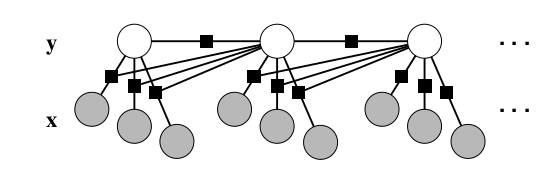
\includegraphics[width=0.7\textwidth]{Bilder/crf-modell-charles-andrew}
%\caption{CRF-Modell (die Abbildung ist der Arbeit von Charles Sutton \cite{Charles/Andrew:10} entnommen)}
%\label{fig:CRF-Modell}
%\end{figure}

%\paragraph{}
%Die Formel, die die Verteilung $p(y|x)$ beschreibt, lautet 
%$$
%p(y|x) = \frac{1}{Z(x)}\prod_{t=1}^T\exp \lbrace \sum_{k=1}^K \theta_k f_k(y_t,y_t-1,x_t) \rbrace
%$$  

%Funktion $f_k$ beschreibt dabei Features, und Vektor $\theta$ - Parameter. Die Funktion $Z(x)$ ist eine Normalisierungsfunktiuon, und wird wie folgt definiert:
%$$
%Z(x) = \sum_y \prod_{t=1}^T\exp \lbrace \sum_{k=1}^K \theta_k f_k(y_t,y_t-1,x_t) \rbrace
%$$
%Vektor $x_t$ beinhaltet dabei alle Features, die benötigt werden, um Abhängigkeiten zu berechnen. 

%\paragraph{}
%Aber wie definiert man Features? Jenny Finkel\cite{Jenny/etal:07} hat folgende Eigenschaften definiert:
%\begin{enumerate}
%\item Nachbarnwörter: vorheriges Wort, nächstes Wort, alle Wörter innerhalb eines Fensters.
%\item Orthographische Eigenschaften.
%\item Präfixe und Suffixe.
%\item Labelsequenzen.
%\end{enumerate}

\subsection{Maximum Entropy based NER}
Was ist ME NER? Wo wird er verwendet? Welche Vor- und Nachteile hat dieser Einsatz im Vergleich zum CRF?
%\paragraph{}
%Dieser Framework wurde in der Arbeit von Andrew Borthwick\cite{Andrew:99} vorgestellt. In diesem Modell wird auch wie im CRF mit der Wahrscheinlichkeit $p(y|x)$ gearbeitet, allerdings ist ME NER kein graphischer Framework. Die Formell, die die Verteilung für ME-Modell beschreibt, sieht wie folgt aus:
%$$
%P(y|x) = \frac{1}{Z(x)}\prod_i \alpha_i^{g_i(x,y)}
%$$
%$g_i$ ist eine binäre Funktion, die eine bestimmte Feature beschreibt, und $\alpha_i$ ist das Parameter, der mit der Eigenschaft assoziiert wird. $Z(x)$ ist eine Normalisierungsfunktion, die wie folgt aussieht:
%$$
%Z(x) = \sum_y \prod_i \alpha_i^{g_i(x,y)}
%$$
%Eigenschaften $g_i$ können in zwei Klassen geteilt werden: lokale und globale Features. Hai und Hwee\cite{Hai/Hwee:02} definieren unter anderem folgende Eigenschaften, die auch im OpenNLP-Framework eingesetzt werden:
%\begin{enumerate}
%\item Globale Eigenschaften:
%\begin{enumerate}
%\item Personenpräfixe für bestimmtes Wort in anderen Sätzen des Dokumentes: z.B. wenn wir im Text zuerst die Tokens ,,Frau Sony`` treffen, und dann einfach ,,Sony``, dann soll angenommen werden, dass ,,Sony`` eine Entität mit dem Typ ,,Person`` ist.
%\item Abkürzungen: wenn in einem Satz mehr Wörter nacheinander groß geschrieben werden, wie z.B. ,,Deutsche Demokratische Republik``, dann wird in dem Text nach entsprechender Abkürzung gesucht: ,,DDR``, und wenn Abkürzung eine Entität ist, können auch alle entsprechende Tokens als eine Entität markiert werden.
%\end{enumerate}
%\item Lokale Eigenschaften:
%\begin{enumerate}
%\item Ob das Wort großgeschrieben wird.
%\item Ob vorheriges oder nächstes Wort großgeschrieben wird.
%\item Ob alle Zeichen im Token großgeschrieben werden.
%\item Ob es ein Punkt am Ende des Wortes steht.
%\item Ob der Token Zahlen beinhaltet, und falls ja, wie viel.
%\item Ob das Wort das Prozent- oder Dollarzeichen beinhaltet.
%\item Suffixe und Präfixe (wie ,,Frau`` oder ,,GmbH``).
%\end{enumerate}
%\end{enumerate}

\section{Wissendatenbanke}
Was sind Wissendatenbanke? Wieso brauchen wir die in unserer Arbeit? Wie sucht man nach Entitäten in einer Wissendatenbank? Kurze Einleitung in SPARQL+RDF.
\paragraph{}
%Um die extrahierte Entitäten mit Ontologien anzureichern, braucht man selbstverständlich eine Datenbank, wo alle Informationen zu den Entitäten gespeichert werden. Solche Datenbanken nennt man ,,Wissendatenbanken``. Solche Datenbanke sind keine herkömmliche relationale Datenbanke, da man die Ontologien mit ihrer hierarchischen Struktur zwar auf ein relationales Modell abbilden lassen kann, aber es gibt bessere Datenstrukturen und Anfragesprachen, die die Arbeit mit Ontologien für die Entwickler einfacher machen.

\paragraph{}
%Zur Beschreibung von Ontologien dient das RDF-Format\footnote{\url{http://www.w3.org/2001/sw/wiki/RDF}}. Dieses Format basiert auf XML, und gibt dem Entwickler eine einfache Möglichkeit, Hierarchische Daten zu beschrieben. Die Ontologie im RDF-Format kann z.B. wie folgt aussehen:
%\lstset{language=XML}
%\lstinputlisting[captionpos=b,label={lst:RDFBEISPIEL},caption={Beispiel einer Ontologie im RDF-Format}]{Listings/examplerdf.xml}

\paragraph{}
%Als Anfragesprache für RDF wird SPARQL\footnote{\url{http://www.w3.org/2001/sw/wiki/SPARQL}} eingesetzt. Diese Sprache sieht SQL ähnlich aus, operiert allerdings nicht auf relationalen Daten, sondern auf RDF-Graphen. 

%Zum Beispiel, wenn die Fläche der Stadt Duisburg und das Bundesland, wo die Stadt liegt, gebraucht werden, kann die SPARQL-Anfrage wie folgt aussehen:
%\lstset{language=SPARQL}
%\lstinputlisting[captionpos=b,label={lst:SPARQLBEISPIEL},caption={Beispiel einer SPARQL-Anfrage}]{Listings/sparqlexample.sql}

%Die Antwort wird dann als RDF-Datensatz geliefert:
%\lstset{language=XML}
%\lstinputlisting[captionpos=b,label={lst:SPARQLRESULT},caption={Beispiel der Antwort auf eine SPARQL-Anfrage}]{Listings/sparqlresult.xml}